\documentclass{beamer}
\usepackage[all]{xy}
\usepackage[utf8x]{inputenc}
\usepackage{default}
\usepackage{verbatim}

\title{AP2DX}
\subtitle{Awesomizing the P2DX}
\author{Jasper Timmer, Maarten Inja, Maarten de Waard, Wadie Assal}
\institute{UvA}
\usetheme{Warsaw}

\begin{document}
\begin{frame}
\titlepage
\end{frame}



\section{Introduction}
\begin{frame}
\frametitle{Introduction}
\begin{itemize}
\item The same assignment
\item Who we are
%Hier dacht ik aan alvast vertellen over Unit tests
\item What is special in our case
\end{itemize}
\end{frame}


\begin{frame}
\frametitle{Goals}
\begin{itemize}
\item Loosely coupled modules based on network communication
\item Robot should be safe, i.e. stop for obstacles
\item Robot should be able to drive autonomously through the environment
\item Robot should be able to create a map of the environment
\item No user input will be required
\end{itemize}
\end{frame}

\section{Architecture}
\subsection{Framework}
\begin{frame}
\frametitle{Architecture - the basics}
\xymatrix{& USARSim \ar@/_/[d] &  \\
& Coordinator \ar@/_/[u] \ar[dr] & \\
Abstract Motor \ar[ur] & Reflex \ar[l]  & Sensor \ar[l] \ar[d] \\
& Planner \ar[u] & Mapper \ar[l] }
\end{frame}


\begin{frame}
\frametitle{Architecture - into the depths}
%\\\\\\
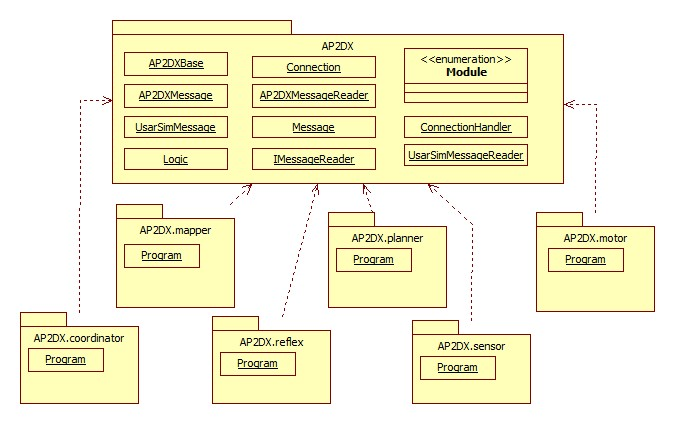
\includegraphics[width=.8\paperwidth]{AP2DX}
\end{frame}

\begin{frame}
\frametitle{Abstract base class}
We decided to use an abstract class, to base all our classes on.
\begin{block}{Advantages}
\begin{itemize}
\item Very easy to work with
\item Only have to make the connection protocol once
\item Strict contracts with team mates
\end{itemize}
\end{block}
\begin{block}{Disadvantages}
\begin{itemize}
\item Stuck with one language
\item Hard debugging
\item Hard to make big changes, or add things we had not thought of
\end{itemize}
\end{block}
\end{frame}

\subsection{Avoiding collision and driving}
\begin{frame}
\frametitle{boobs}
%TODO: I DON"T KNOW HOW THIS WORKS!!
\end{frame}

\subsection{Creating a map}
\begin{frame}
\frametitle{Mapper}
We did not make our own mapper. We used DP
Slam\footnote{http://www.cs.duke.edu/~parr/dpslam/}\footnote{Algorithm from: Austin Eliazar,
Ronald Parr: DP-SLAM: Fast, Robust Simultainous Localization and Mapping Without
Predetermined Landmarks}.\\
The program works in C, and creates a map like this one:

\includegraphics[height=.5\textheight]{hmap00}
\end{frame}

\begin{frame}
\frametitle{Mapper - What makes it special}
\begin{itemize}
    \item Two ways to use a mapper:
    \begin{itemize}
        \item While driving
        \item After driving (with saved sensordata)
    \end{itemize}
    \item We make a map, while driving
    \item Mapper uses Odometry and Laser range scanner data
    \item Currently only works on linux
    \end{itemize}
\end{frame}

\subsection{Communication}
\begin{frame}
\frametitle{Messages}
\xymatrix{& Message \ar[dl] \ar[dr] &  \\
AP2DXMessage \ar[d] && UsarSimMessage \ar[d] & \\
SpecializedMessage\ar[d] && (individual messages) \\
(individual messages)& &  }
\end{frame}

\begin{frame}
\frametitle{Messages - explained}
There are a couple of advantages and disadvantages:
\begin{block}{Advantages}
\begin{itemize}
\item Very easy to work with
\item Easy to add a new kind of message
\item Strict restrictions to how a message should look (and thus uniformity)
\end{itemize}
\end{block}

\begin{block}{Disadvantages}
\begin{itemize}
\item Very hard to debug
\item Hard to add a type of message that doesn't fit in
\end{itemize}
\end{block}
\end{frame}

\section{Testing and jUnit}
\begin{frame}
\frametitle{Testing - an introduction}
We decided to use jUnit tests, since all our code is in Java.\\
For this, we used Jenkins, an automatic build and test server\\
\end{frame}


{
     \usebackgroundtemplate{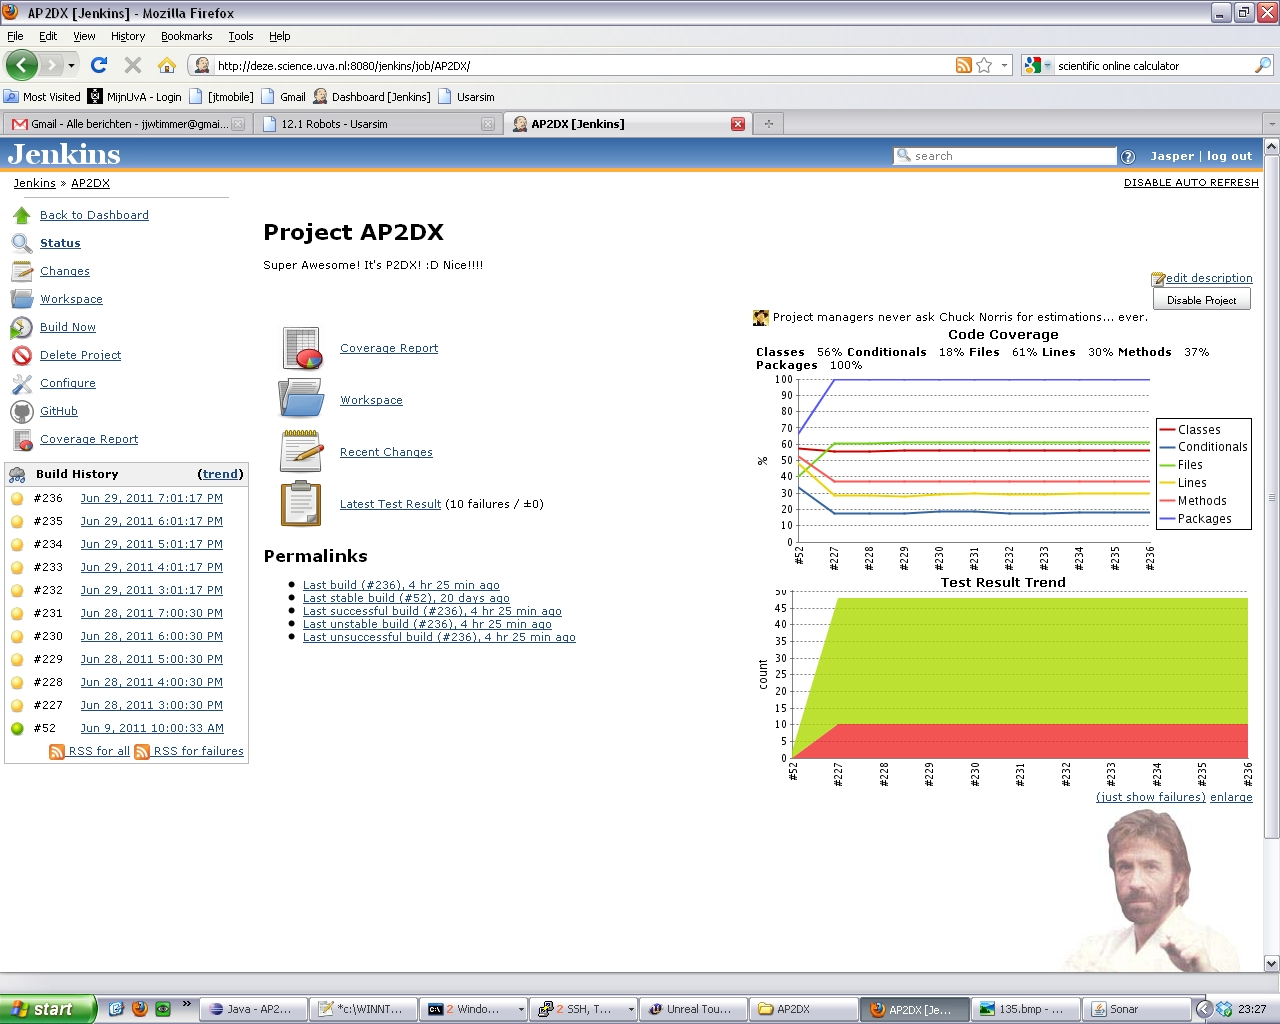
\includegraphics[width=\paperwidth]{jenkins_project}} 
      \begin{frame}
      \end{frame}
}

{
     \usebackgroundtemplate{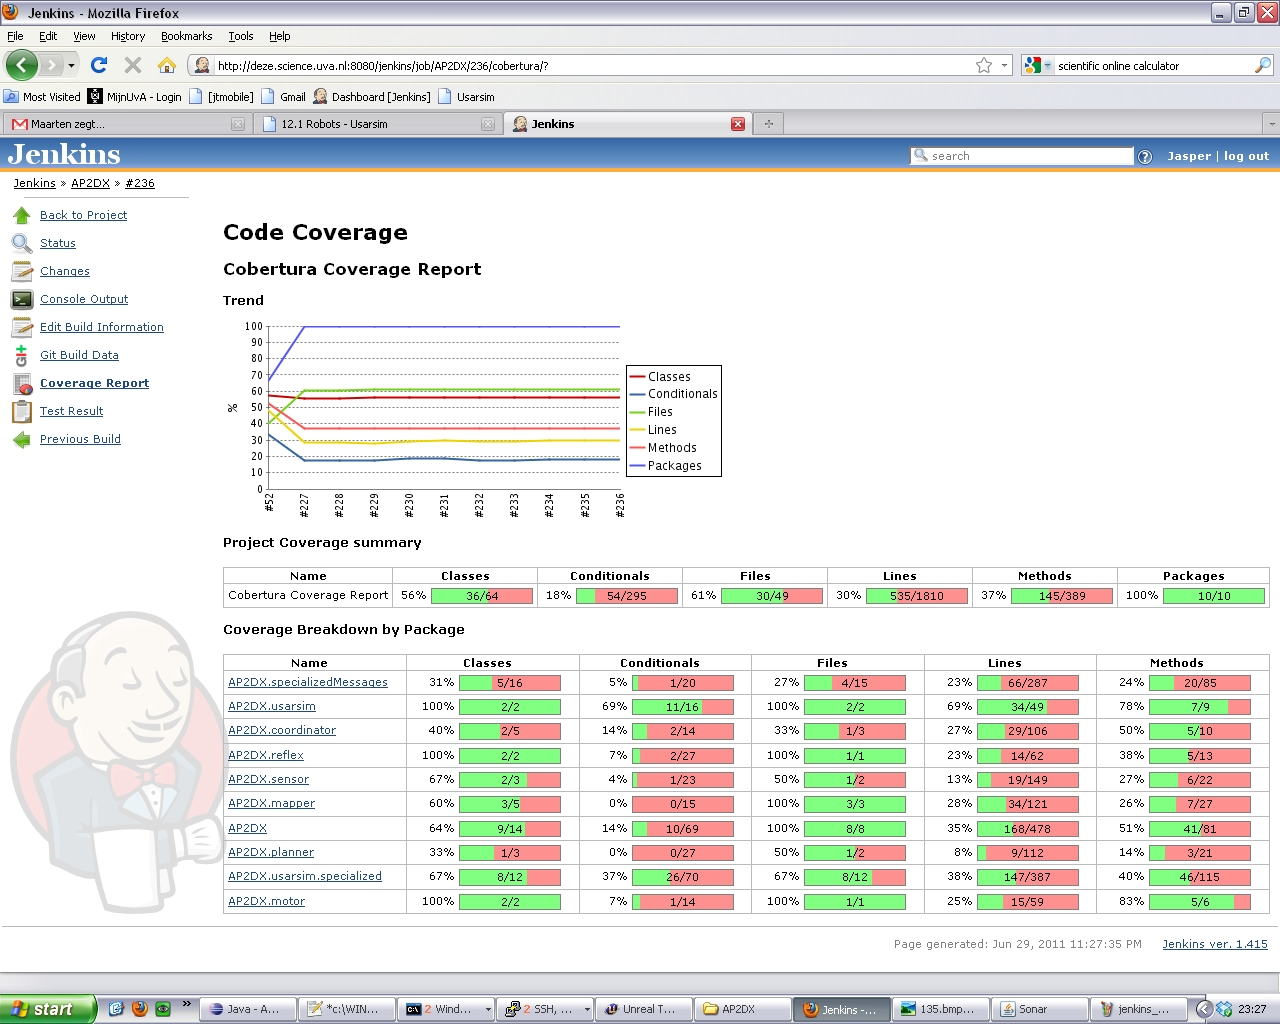
\includegraphics[width=\paperwidth]{jenkins_coverage}} 
      \begin{frame}
      \end{frame}
}
{
     \usebackgroundtemplate{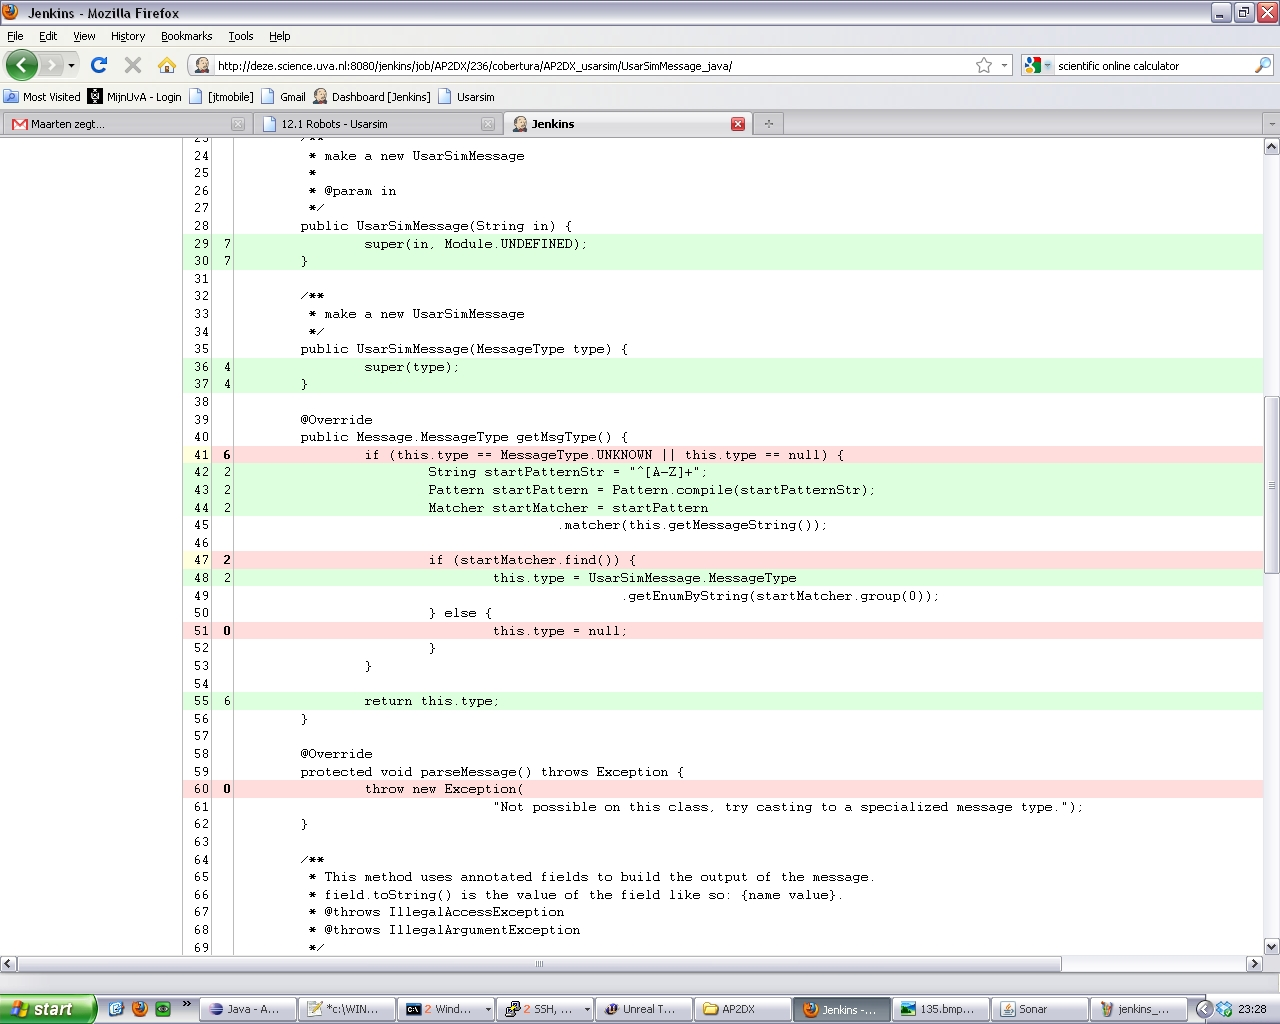
\includegraphics[width=\paperwidth]{jenkins_linecoverage}} 
      \begin{frame}
      \end{frame}
}


\section{Problems \& Solutions}

\end{document}
